\section{Differential KV Compression}
\label{sec:compression}

\begin{figure}[t]
  \centering
  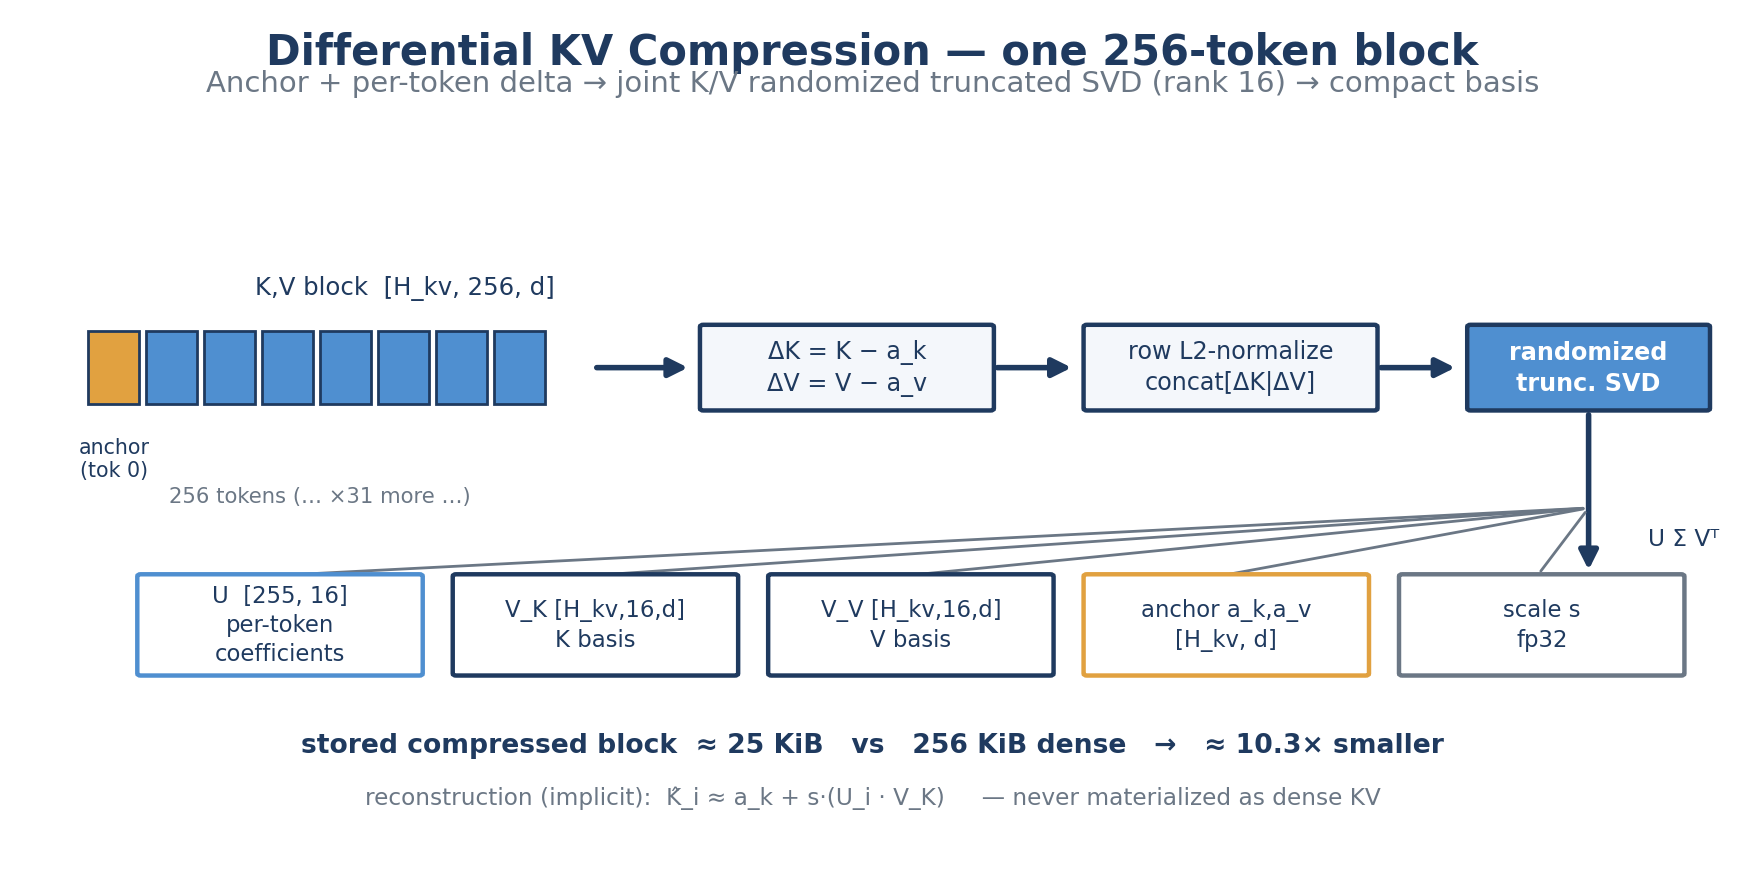
\includegraphics[width=\linewidth]{figures/f2_compression.png}
  \caption{Compressing one $256$-token block. The first token is the anchor; the remaining
  $255$ tokens are represented as their deviations from it. Keys and values are stacked and
  jointly factorized by a rank-$16$ randomized truncated SVD, yielding a shared per-token
  coefficient matrix $U$ and separate key/value bases $V_K,V_V$. The block shrinks from
  $256$\,KiB to $\approx\!25$\,KiB per layer.}
  \label{fig:compress}
\end{figure}

\subsection{Notation}
Within one layer, a block of $\bs{=}256$ contiguous tokens has keys
$K\in\R^{\Hkv\times \bs\times \dhead}$ and values $V$ of the same shape
($\Hkv{=}2$, $\dhead{=}128$). We compress blocks independently and per layer.

\subsection{Anchor + differential representation}
The first token of the block is the \emph{anchor}; per head $h$ we keep its key and value
exactly:
\begin{equation}
\anchork^{(h)} = K^{(h)}_{0}, \qquad \anchorv^{(h)} = V^{(h)}_{0}.
\end{equation}
For the remaining $S{=}\bs-1$ tokens we form deltas against the anchor,
\begin{equation}
\Delta K^{(h)}_{i} = K^{(h)}_{i} - \anchork^{(h)}, \quad
\Delta V^{(h)}_{i} = V^{(h)}_{i} - \anchorv^{(h)}, \quad i=1{\dots}S,
\end{equation}
and stack them across heads into a single matrix per modality. Concatenating keys and values
gives the joint delta matrix
\begin{equation}
X = \big[\,\Delta K \;\big|\; \Delta V\,\big]\in\R^{S\times 2\Hkv\dhead},
\label{eq:X}
\end{equation}
i.e. $X\in\R^{255\times 512}$ here. Joint factorization is deliberate: it forces keys and
values of the same token to share one low-rank coefficient vector, halving the per-token
coefficient storage relative to factorizing them separately.

\subsection{Normalized randomized truncated SVD}
Tokens within a block differ widely in delta magnitude, and an unnormalized SVD spends its
budget on the largest-norm rows. We therefore $\ell_2$-normalize each row before
factorization, storing the norms separately:
\begin{equation}
n_i = \lVert X_i\rVert_2,\qquad \hat X_i = X_i / \max(n_i,\,\epsilon).
\end{equation}
$\hat X$ is then factorized by a randomized truncated SVD~\cite{halko2011randomized} at target
rank $\rank{=}16$: a global scale $s=\max|\hat X|$ is divided out, an oversampled Gaussian
range finder ($\rank{+}5$ columns) with two power iterations and a QR step yields an
orthonormal basis $Q$, and a small projected SVD of $Q^{\!\top}\hat X$ gives
$\hat X \approx U_k\Sigma_k V_k^{\!\top}$. An \emph{adaptive} rank keeps the fewest components
explaining $99.9\%$ of the spectral energy, clamped to $[4,\rank]$. The stored factors are
\begin{equation}
U = (U_k\Sigma_k)\odot n \in\R^{S\times \rank},\qquad
V^{\!\top} = V_k^{\!\top}\in\R^{\rank\times 2\Hkv\dhead},
\end{equation}
where the row-norms $n$ are re-applied to $U$ so that reconstruction recovers the true delta
scale. $V^{\!\top}$ is split back into key and value bases $V_K,V_V\in\R^{\Hkv\times\rank\times\dhead}$.
The block is stored as $(U,V_K,V_V,\anchork,\anchorv,s)$ in fp16 (scale $s$ in fp32). The
implicit reconstruction of any token---never materialized in practice---is
\begin{equation}
\hat K^{(h)}_i \;\approx\; \anchork^{(h)} + s\,\big(U_i\, V_K^{(h)}\big),
\label{eq:recon}
\end{equation}
and analogously for values. We run the SVD in NumPy: on unified memory the array is the same
bytes the GPU uses, so the only cost is compute, and a $255{\times}512$ factorization is a few
milliseconds---amortized over the $256$ tokens it represents.

\begin{algorithm}[t]
\caption{\textsc{CompressBlock} (one block, one layer)}
\label{alg:compress}
\begin{algorithmic}[1]
\Require block keys $K$, values $V$ $\in\R^{\Hkv\times \bs\times \dhead}$; rank $\rank$
\State $\anchork \gets K_{:,0,:};\ \anchorv \gets V_{:,0,:}$
\State $\Delta K \gets K_{:,1:,:}-\anchork;\quad \Delta V \gets V_{:,1:,:}-\anchorv$
\State $X \gets \textsc{StackHeads}([\Delta K \mid \Delta V])$ \Comment{$\R^{S\times 2\Hkv\dhead}$}
\State $n_i \gets \lVert X_i\rVert_2;\quad \hat X \gets X / n$ \Comment{row normalize}
\State $U_k,\Sigma_k,V_k,s,k \gets \textsc{RandTruncSVD}(\hat X,\rank)$ \Comment{adaptive $k\le\rank$}
\State $U \gets (U_k\Sigma_k)\odot n;\quad [V_K\mid V_V]\gets V_k^{\!\top}$
\State pad $U$ to $\R^{S\times\rank}$, $V$ to rank $\rank$; \Return $(U,V_K,V_V,\anchork,\anchorv,s)$
\end{algorithmic}
\end{algorithm}

\subsection{Storage budget and complexity}
Table~\ref{tab:budget} gives the exact per-block byte budget. The compressed block stores the
shared coefficients $U$ ($S\rank$), two bases $V_K,V_V$ ($2\Hkv\rank\dhead$), two anchors
($2\Hkv\dhead$), and two scalars---$25{,}576$ bytes against $262{,}144$ for the dense block,
a $\mathbf{10.25\times}$ reduction at equal (fp16) precision.

\begin{table}[t]
\centering
\caption{Per-$256$-token-block storage budget (one layer, fp16). Derived from the model
dimensions ($\Hkv{=}2$, $\dhead{=}128$) and configuration ($\bs{=}256$, $\rank{=}16$).}
\label{tab:budget}
\small
\begin{tabular}{lrr}
\toprule
Component & DiffKV block & Dense block \\
\midrule
$U$ coefficients $[255,16]$ fp16 & 8160 B & -- \\
$V_K,V_V\ [2,16,128]$ fp16 & 16384 B & -- \\
anchors $a_k,a_v\ [2,128]$ fp16 & 1024 B & -- \\
key min/max $[2,128]$ fp16 (router) & 1024 B & -- \\
scale + seq\_len & 8 B & -- \\
\textbf{residual $K,V\ [64,2,128]$ fp16} & \textbf{65536 B} & -- \\
full $K,V\ [256,2,128]$ fp16 & -- & 262144 B \\
\midrule
\textbf{Per 256-token block} & \textbf{90.0 KiB} & \textbf{256 KiB} \\
Compression ratio & \multicolumn{2}{c}{$2.85\times$} \\
\bottomrule
\end{tabular}
\end{table}

\noindent
Asymptotically, a compressed block costs $O(\bs\rank + \Hkv\rank\dhead)$ versus the dense
$O(\bs\Hkv\dhead)$; with $\rank \ll \Hkv\dhead$ the per-token term $\bs\rank$ dominates, so the
\emph{marginal} cost of a token in the compressed pool is $O(\rank)$ scalars rather than
$O(\Hkv\dhead)$. This $\rank$-vs-$\Hkv\dhead$ gap (here $16$ vs $256$) is the source of the
bounded-memory behavior in \S\ref{sec:runtime}. The factorization itself is
$O(S\cdot 2\Hkv\dhead\cdot \rank)$ per block and fires once per $\bs$ tokens, so its amortized
per-token compute is $O(\Hkv\dhead\rank)$---the prefill cost we quantify in \S\ref{sec:eval}.
